%% appendix

\section{The Equipartition theorem and the Fluctuation dissapation theorem}

\newpage

%input{notes/crystal_classification_table}

\section{AlGaAs coating orientation to beam polarization}

\begin{figure*}
    \begin{subfigure}{\includegraphics[width=.5\textwidth]{figs/ALGAAS/coating_orientation_normal.png}}
    \end{subfigure}
    \hfill
    \begin{subfigure}{\includegraphics[width=.5\textwidth]{figs/ALGAAS/coating_orientation_isometric.png}}
    \end{subfigure}

    \caption{\textcolor{red}{PENDING UPDATES Laser orientation with respect to the beam axis (isometric and normal views)}}
    \label{fig:algaas_beam_orienation_blender_1}
\end{figure*}

\section{Mode matching data for Electro-optic sample cavity}
\subsection{Pre MMT beam scan}

\begin{figure}[H]
\includegraphics[width=\textwidth]{figs/ALGAAS/beamscans/12_18_2020_preMMT.png}
\caption{Beam scan taken from SM5 (Steering mirror 5)}
\label{fig:macor_mount_design}
\end{figure}


\subsection{``Just another mode matching tool" (JAMMT) solution}


\subsection{Post MMT beam scan}

\begin{figure}[H]
\includegraphics[width=\textwidth]{figs/ALGAAS/beamscans/01_12_2021_postMMT.png}
\caption{Beam scan taken from SM6. Sampling points before SM7 and after the first cavity iris.}
\label{fig:macor_mount_design}
\end{figure}

\subsection{Laser PZT sweep}



\section{Calibration}\label{sec:calibration_math}
The frequency response measurement shown in (?) records the following transfer function in dB of the following:

\begin{equation}
\alpha(f) = \frac{\mathrm{CH2}(f)}{Source}
\end{equation}

Channel

We also know that the error signal spectra of the loop is probed by $CH2(f)$:


\begin{equation}
\mathrm{CH2}(f) = \frac{\mathrm{S}(f)*signal_V}{(1-\mathrm{OLG}(f))}
\end{equation}

Where $signal_V$ is the uncalibrated voltage output from the mixer, $\mathrm{S}(f)$ is the FSS transfer function, and $\mathrm{OLG}(f)$ is the open loop gain of the PDH system.

And we know $\mathrm{OLG}(f) = \mathrm{S}(f)*\mathrm{A}(f)$ so :

\begin{equation}
\mathrm{signal}_m = \mathrm{CH2}(f)*\mathrm{A}(f) \frac{1-\mathrm{OLG}(f)}{\mathrm{OLG}(f)} \frac{L_\mathrm{cav}}{f_\mathrm{laser}}
\end{equation}

Where $\mathrm{A}*(f)$ is the high voltage amplifier response with the Mephisto 2220 laser PZT response. $L_\mathrm{cav}$ is the sample cavity length, $f_\mathrm{laser}$ is the laser frequency. ($\mathrm{signal}_m$)  is the effective cavity length change from the Pockels effect.

Substitute (1) into (4):

\begin{equation}
\mathrm{signal}_m = \mathrm{Source} * \alpha(f) * \mathrm{A}(f) \frac{1-\mathrm{OLG}(f)}{\mathrm{OLG}(f)} \frac{L_\mathrm{cav}}{f_\mathrm{laser}}
\end{equation}

Measured :
Source, $\alpha (f)$, OLG$(f)$, A$(f)$ and $L_\mathrm{cav}$

\section{Laplace calculator / code}

\textcolor{red}{Snippets of explicit code with a block diagram for clarity}

\section{MACOR assembly}

\begin{figure}[H]
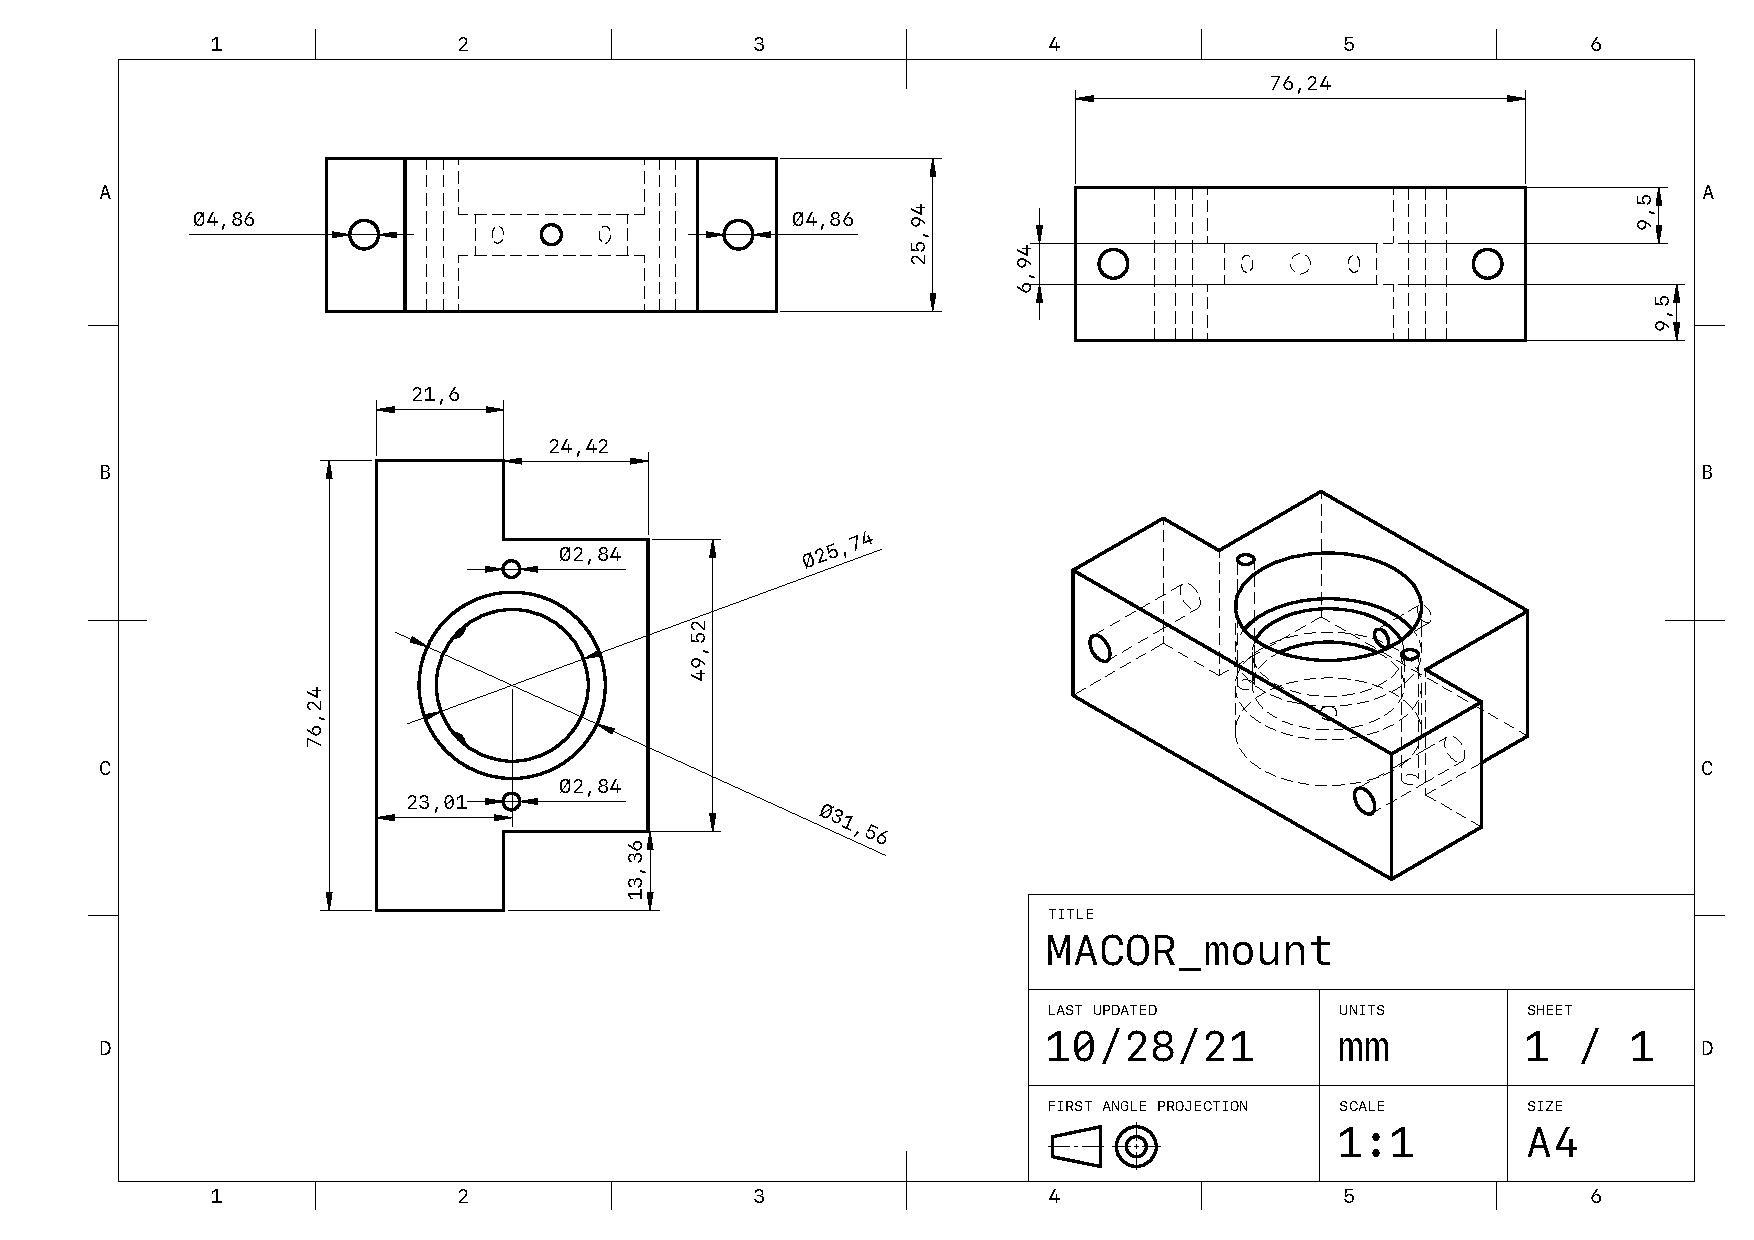
\includegraphics[width=\textwidth]{figs/ALGAAS/MACOR_mount.pdf}
\caption{MACOR mount design constucted in Shapr3D}
\label{fig:macor_mount_design}
\end{figure}

\section{HVA}






\section{FSS}



\begin{figure}[H]
\includegraphics[width=\textwidth]{figs/ALGAAS/tfs/spice_FSS_tf.png}
\caption{The FSS frequency response simulated in LTspice}
\label{fig:spiceFSS}
\end{figure}
